%%%%%%%%%%%%%%%%%%%%%%%%%%%%%%%%%%%%%%%%%%%%%%%%%%%%%%%%%%%%%%%%%%%%%%%%%%%%%%%%
%% Title (en): Multiagent Systems and Organizations                           %%
%% Title (cs): Multiagentní systémy a organizace                              %%
%%                                                                            %%
%% Author: Bc. Lukáš Kúdela                                                   %%
%% Supervisor: Prof. RNDr. Petr Štěpánek, DrSc.                               %%
%%                                                                            %%
%% Academic year: 2011/2012                                                   %%
%%%%%%%%%%%%%%%%%%%%%%%%%%%%%%%%%%%%%%%%%%%%%%%%%%%%%%%%%%%%%%%%%%%%%%%%%%%%%%%%

%%%%%%%%%%%%%%%%%%%%%%%%%%%%%%%%%%%%%%%%%%%%%%%%%%%%%%%%%%%%%%%%%%%%%%%%%%%%%%%%
\section{Example 3: Auction}
%%%%%%%%%%%%%%%%%%%%%%%%%%%%%%%%%%%%%%%%%%%%%%%%%%%%%%%%%%%%%%%%%%%%%%%%%%%%%%%%

%%%%%%%%%%%%%%%%%%%%%%%%%%%%%%%%%%%%%%%%%%%%%%%%%%%%%%%%%%%%%%%%%%%%%%%%%%%%%%%%
\subsection*{Specification}

%%%%%%%%%%%%%%%%%%%%%%%%%%%%%%%%%%%%%%%%%%%%%%%%%%%%%%%%%%%%%%%%%%%%%%%%%%%%%%%%
\subsubsection*{Organization Part}

% Auction organization
This example demonstrates a relatively complex organization - the \textit{Auction} organization (modelled by the \texttt{Auction\_Organization} agent class).
% Auction organization - purpose
The purpose of the organization is to facilitate an auction by grouping three or more agents: one agent \textit{auctions} an item and the other agents \textit{bid} for it.
The item can be auctioned in an envelope, Vickrey, english or dutch auction.
The example uses the envelope auction to sell works of art, but it should be apparent that any of the four auction types can be used to sell any items.

% Auction organization - roles
The \textit{Auciton} organization has two roles - \textit{Auctioneer} and \textit{Bidder} - and four protocols - \textit{Envelope auction}, \textit{Vickrey auction}, \textit{English auction} and \textit{Dutch auction}.

% Auctioneer role
The \textit{Auctioneer} role (modelled by the \texttt{Auctioneer\_Role} class) is a single role representing an auctioneer in an auction.
The auctioneer is an auction participant trying to sell the auctioned item.
There is only one auctioneer, hence the single role.
% Auctioneer role - competences & responsibilities
The \textit{Auctioneer} has one competence - \textit{Auction} - and no responsibilities.

% Auction competence
The \textit{Auction} competence (modelled by the \texttt{Auction\_Competence} class) is a competence to auction an item.
% Auction competence - argument & result
The competence has several arguments - TODO - and several results - TODO.

% Bidder role
The \textit{Bidder} role (modelled by the \texttt{Bidder\_Role} class) is a multiple role representing a bidder in an auction.
A bidder is an auction participant attempting to buy the auctioned item.
There are many bidders, hence the multiple role.
% Bidder role - competences & responsibilities
It has no competences and one responsibility - \textit{Bid}.

% Bidder responsibility
The \textit{Bid} responsibility (modelled by the \texttt{Bid\_Responsibility} class) is a responsibility to bid for an item.
% Bidder responsibility - argument & result
The responsibility has several arguments - TODO - and several results - TODO.

%%%%%%%%%%%%%%%%%%%%%%%%%%%%%%%%%%%%%%%%%%%%%%%%%%%%%%%%%%%%%%%%%%%%%%%%%%%%%%%%
\subsubsection*{Protocol Part}

% Envelope acution protocol
The \textit{Envelope auction} protocol (modelled by the \texttt{EnvelopeAuctionProtocol} class) is a protocol defining the Envelope auction.
% Envelope auction
The Envelope auction is a sealed bid first-price auction.
In this type of auction the sealed bids (unknown to other bidders) are submitted simultaneously to the auctioneer and the item is sold to the winning bidder for the price of their bid.

% Vickrey auction protocol
The \textit{Vickrey auction} protocol (modelled by the \texttt{VickreyAuctionProtocol} class) is a protocol defining the Vickrey auction.
% Vickrey auction
The Vickrey auction is a sealed bid second-price auction.
In this type of auction the sealed bids are submitted simultaneously to the auctioneer and the item is sold to the winning bidder for the price of the \textit{second} highest bid.

% English auction protocol
The \textit{English auction} protocol (modelled by the \texttt{EnglishAuctionProtocol} class) is a protocol defining the English auction. 
% English auction
The English auction is an open bid ascending price auction.
In this type of auction the auctioneer announces the starting price (lower than the expected selling price).
The bidders then sequentially submit open bids in ascending fashion, respecting the minimum increment.
The item is sold to the \textit{last} bidder willing to pay the price.

% Dutch auction protocol
The \textit{Dutch auction} protocol (modelled by the \texttt{DutchAuctionProtocol} class) is a protocol defining the Dutch auction.
% Dutch auction
The Dutch auction is an open bid descending price auction.
In this type of auction the auctioneer announces a starting price (higher than the expected selling price).
The auctioneer then sequentially offers prices in descending fashion, respecting the minimum decrement.
The item is sold to the \textit{first} bidder willing to pay the price.

% AuctionCFP message
The \textit{Auction CFP} message (modelled by the \texttt{AuctionCFPMessage}) is a message sent by the \textit{Auctioneer} to all \textit{Bidders} carrying an auction call-for-proposal together with the auctioned item's name.

% Bid message
The \textit{bid} message (modelled by the \texttt{BidMessage}) is a message sent by a \textit{Bidder} to the \textit{Auctioneer} carrying information that a bid has been made together with the bid.

%%%%%%%%%%%%%%%%%%%%%%%%%%%%%%%%%%%%%%%%%%%%%%%%%%%%%%%%%%%%%%%%%%%%%%%%%%%%%%%%
\subsubsection*{Player Part}

% Participant player
The \textit{Participant} player (modelled by the \texttt{Participant\_Player} agent class) is a player capable of bidding in an auction.

%%%%%%%%%%%%%%%%%%%%%%%%%%%%%%%%%%%%%%%%%%%%%%%%%%%%%%%%%%%%%%%%%%%%%%%%%%%%%%%%
\section{Manifestation}

% Agents - players & organizations
There are three \textit{Participant} players in the running MAS - the  \textit{participant1}, \textit{participant2} and \textit{participant3} players (modelled by the \texttt{participant1\_Player}, \texttt{participant2\_Player} and \texttt{participant3\_Player} agent instances respectively) - and one organization - the \textit{Auction} organization (modelled by the \textit{auction\_Organization} agent instance).

% Agent intentions
The intention of each \textit{Participant} player to sell an item (works of art in this example) to one of the other participants - the one who is willing to pay the most.
Here we will reproduce only the first round (\textit{participant1} is the auctioneer); the second and third rounds (with \textit{participant2} and \textit{participant3} as auctioneers respectively) follow the same pattern. 

%%%%%%%%%%%%%%%%%%%%%%%%%%%%%%%%%%%%%%%%%%%%%%%%%%%%%%%%%%%%%%%%%%%%%%%%%%%%%%%%
\subsubsection*{Stage 1: Role Enactment}

% Figure: Stage 1: Role enactment
\begin{figure}[H]
	\centering
	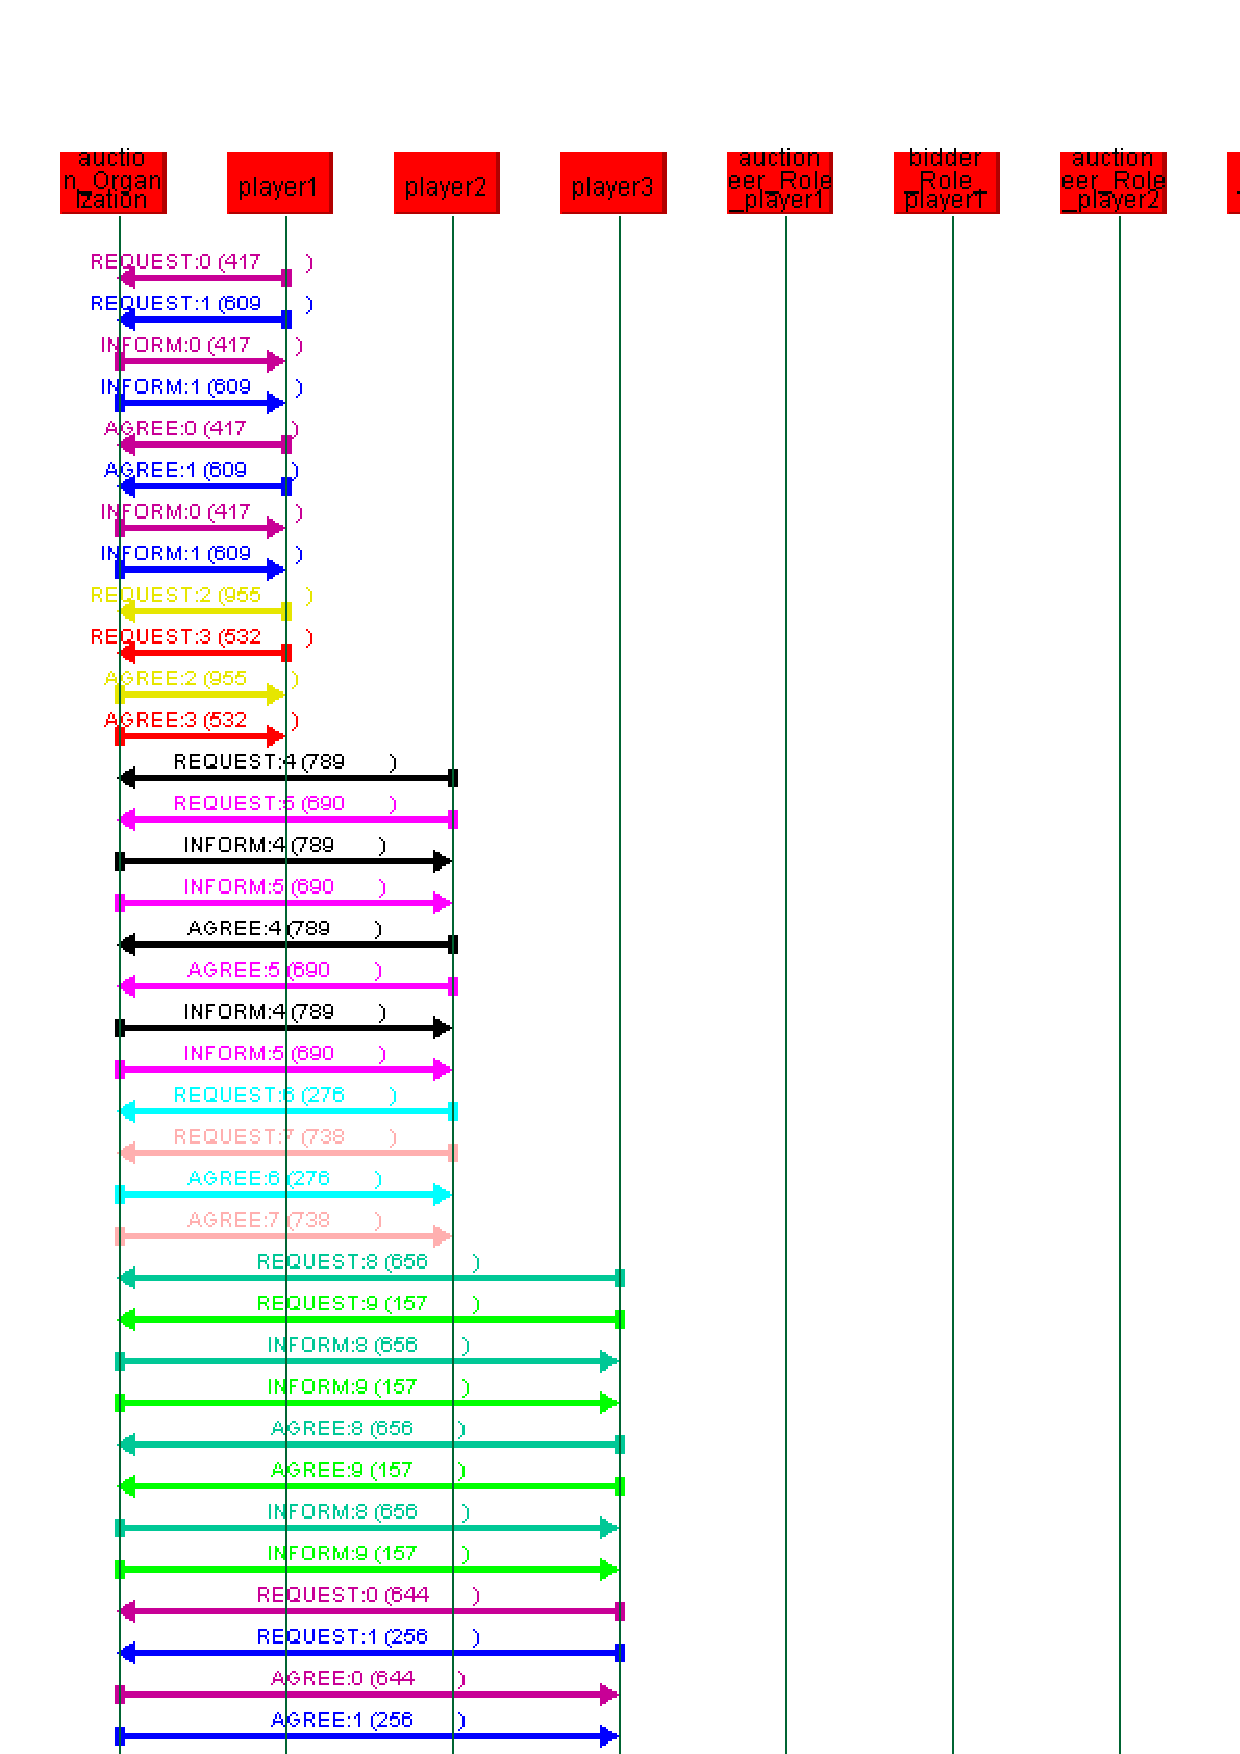
\includegraphics[width=\textwidth]{images/example3-stage1.png}
	\caption{Stage 1: Role enactment}
	\label{figure:example3-stage1}
\end{figure}

% Purple
\textbf{Purple} The purple interaction scenario between the \textit{participant1} player and the \textit{auction} organization follows the \textit{Enact role} protocol.
\textit{participant1} requests \textit{auction} to enact the \textit{Auctioneer} role, which has no responsibilities.

% Gold
\textbf{Gold} The gold interaction scenario between the \textit{participant2} player and the \textit{auction} organization follows the \textit{Enact role} protocol.
\textit{participant2} requests \textit{auction} to enact the \textit{Bidder} role, which has one responsibility - the \textit{Bid} responsibility.

% Blue
\textbf{Blue} The blue interaction scenario between the \textit{participant3} player and the \textit{auction} organization follows the \textit{Enact role} protocol.
\textit{participant3}, like \textit{participant2}, requests \textit{auction} to enact the \textit{Bidder} role.

% Enact role protocol - details
For details of the \textit{Enact role} interaction protocol see Stage 1 of the first example.

%%%%%%%%%%%%%%%%%%%%%%%%%%%%%%%%%%%%%%%%%%%%%%%%%%%%%%%%%%%%%%%%%%%%%%%%%%%%%%%%
\subsubsection*{Stage 2: Role Activation}

% Figure: Stage 2: Role activation
\begin{figure}[H]
	\centering
	\includegraphics[width=\textwidth]{images/example3-stage2.png}
	\caption{Stage 2: Role activation}
	\label{figure:example3-stage2}
\end{figure}

% Red
\textbf{Red} The red interaction scenario between the \textit{participant1} player and the \textit{auctioneer-participant1} position follows the \textit{Activate role} protocol.

% Black
\textbf{Black} The black interaction scenario between the \textit{participant2} player and the \textit{bidder-participant2} position follows the \textit{Activate role} protocol.

% Magenta
\textbf{Magenta} The magenta interaction protocol between the \textit{participant3} player and the \textit{bidder-participant3} position follows the \textit{Activate role} protocol.

% Activate role protocol - details
For details of the \textit{Activate role} interaction protocol see Stage 2 of the first example.

%%%%%%%%%%%%%%%%%%%%%%%%%%%%%%%%%%%%%%%%%%%%%%%%%%%%%%%%%%%%%%%%%%%%%%%%%%%%%%%%
\subsubsection*{Stage 3: Competence and Responsibility Invocation}

% Figure: Stage 3: Competence and responsibility invocation
\begin{figure}[H]
	\centering
	\includegraphics[width=\textwidth]{images/example3-stage3.png}
	\caption{Stage 3: Competence and responsibility invocation}
	\label{figure:example3-stage3}
\end{figure}

% Cyan
\textbf{Cyan} The cyan interaction scenario between the \textit{participant1} player and the \textit{auctioneer-participant1} position follows the \textit{Invoke competence} protocol.
\textit{participant1} requests \textit{auctioneer-participant1} to invoke the \textit{Auction} competence and informs the position about the competence argument - the name of the work of art and the reserve price.
After \textit{auctioneer-participant1} executes the competence (the pink interaction scenario), it informs \textit{participant1} about the competence result - the AID of the winning bidder and the selling price.

% Pink
\textbf{Pink} The pink interaction scenario among the \textit{auctioneer-participant1}, \textit{bidder-participant2} and \textit{bidder-participant3} positions.
\textit{auctioneer-participant1} calls for proposals from \textit{bidder-participant2} and \textit{bidder-participant3} (1\textsuperscript{st} and 2\textsuperscript{nd} messages).
Both \textit{bidder-participant2} and \textit{bidder-participant} then invoke the \textbf{Bid} responsibility on their respective players (the green and teal interaction scenarios respectively) and propose their bids to \textit{auctioneer-participant3} (3\textsuperscript{rd} and 4\textsuperscript{th} messages).
\textit{auctioneer-participant1} then determines the winning bidder, accepts their proposal (5\textsuperscript{th} message) and rejects the other bidders' proposals (6\textsuperscript{th} message).

% Green
\textbf{Green} The green interaction scenario between the \textit{bidder-participant2} position and the \textit{participant2} player follows the \textit{Invoke responsibility} protocol.
\textit{bidder-participant2} requests \textit{participant2} to invoke the \textit{Bid} responsibility and informs the player about the responsibility argument - the name of the work of art.
After \textit{participant2} execute the responsibility, it informs \textit{bidder-participant2} about the responsibility result - the bid.

% Teal
\textbf{Teal} The teal interaction scenario between the \textit{bidder-participant3} position and the \textit{participant3} player follows the \textit{Invoke responsibility} protocol.
This interaction scenario is similar to the green interaction scenario.

% Invoke competence protocol & Invoke responsibility protocol - details
For details about the \textit{Invoke competence} and \textit{Invoke responsibility} protocol see Stage 3 of the first example.

%%%%%%%%%%%%%%%%%%%%%%%%%%%%%%%%%%%%%%%%%%%%%%%%%%%%%%%%%%%%%%%%%%%%%%%%%%%%%%%%
\subsubsection*{Stage 4: Role Deactivation}

% Figure: Stage 4: Role deactivation
\begin{figure}[H]
	\centering
	\includegraphics[width=\textwidth]{images/example3-stage4.png}
	\caption{Stage 4: Role deactivation}
	\label{figure:example3-stage4}
\end{figure}

% Blue
\textbf{Blue} The gold interaction scenario between the \textit{participant1} player and the \textit{auctioneer-participant1} position follows the \textit{Deactivate role} protocol.

% Purple
\textbf{Purple} The purple interaction scenario between the \textit{participant2} player and the \textit{bidder-participant2} position follows the \textit{Deactivate role} protocol.

% Gold
\textbf{Gold} The gold interaction scenario between the \textit{participant3} player and the \textit{bidder-participant3} position follows the \textit{Deactivate role} protocol.

% Deactivate role protocol - details
For details of the \textit{Deactivate role} interaction protocol see Stage 4 of the first example.

%%%%%%%%%%%%%%%%%%%%%%%%%%%%%%%%%%%%%%%%%%%%%%%%%%%%%%%%%%%%%%%%%%%%%%%%%%%%%%%%
\subsubsection*{Stage 5: Role Deactment}

% Figure: Stage 5: Role deactment
\begin{figure}[H]
	\centering
	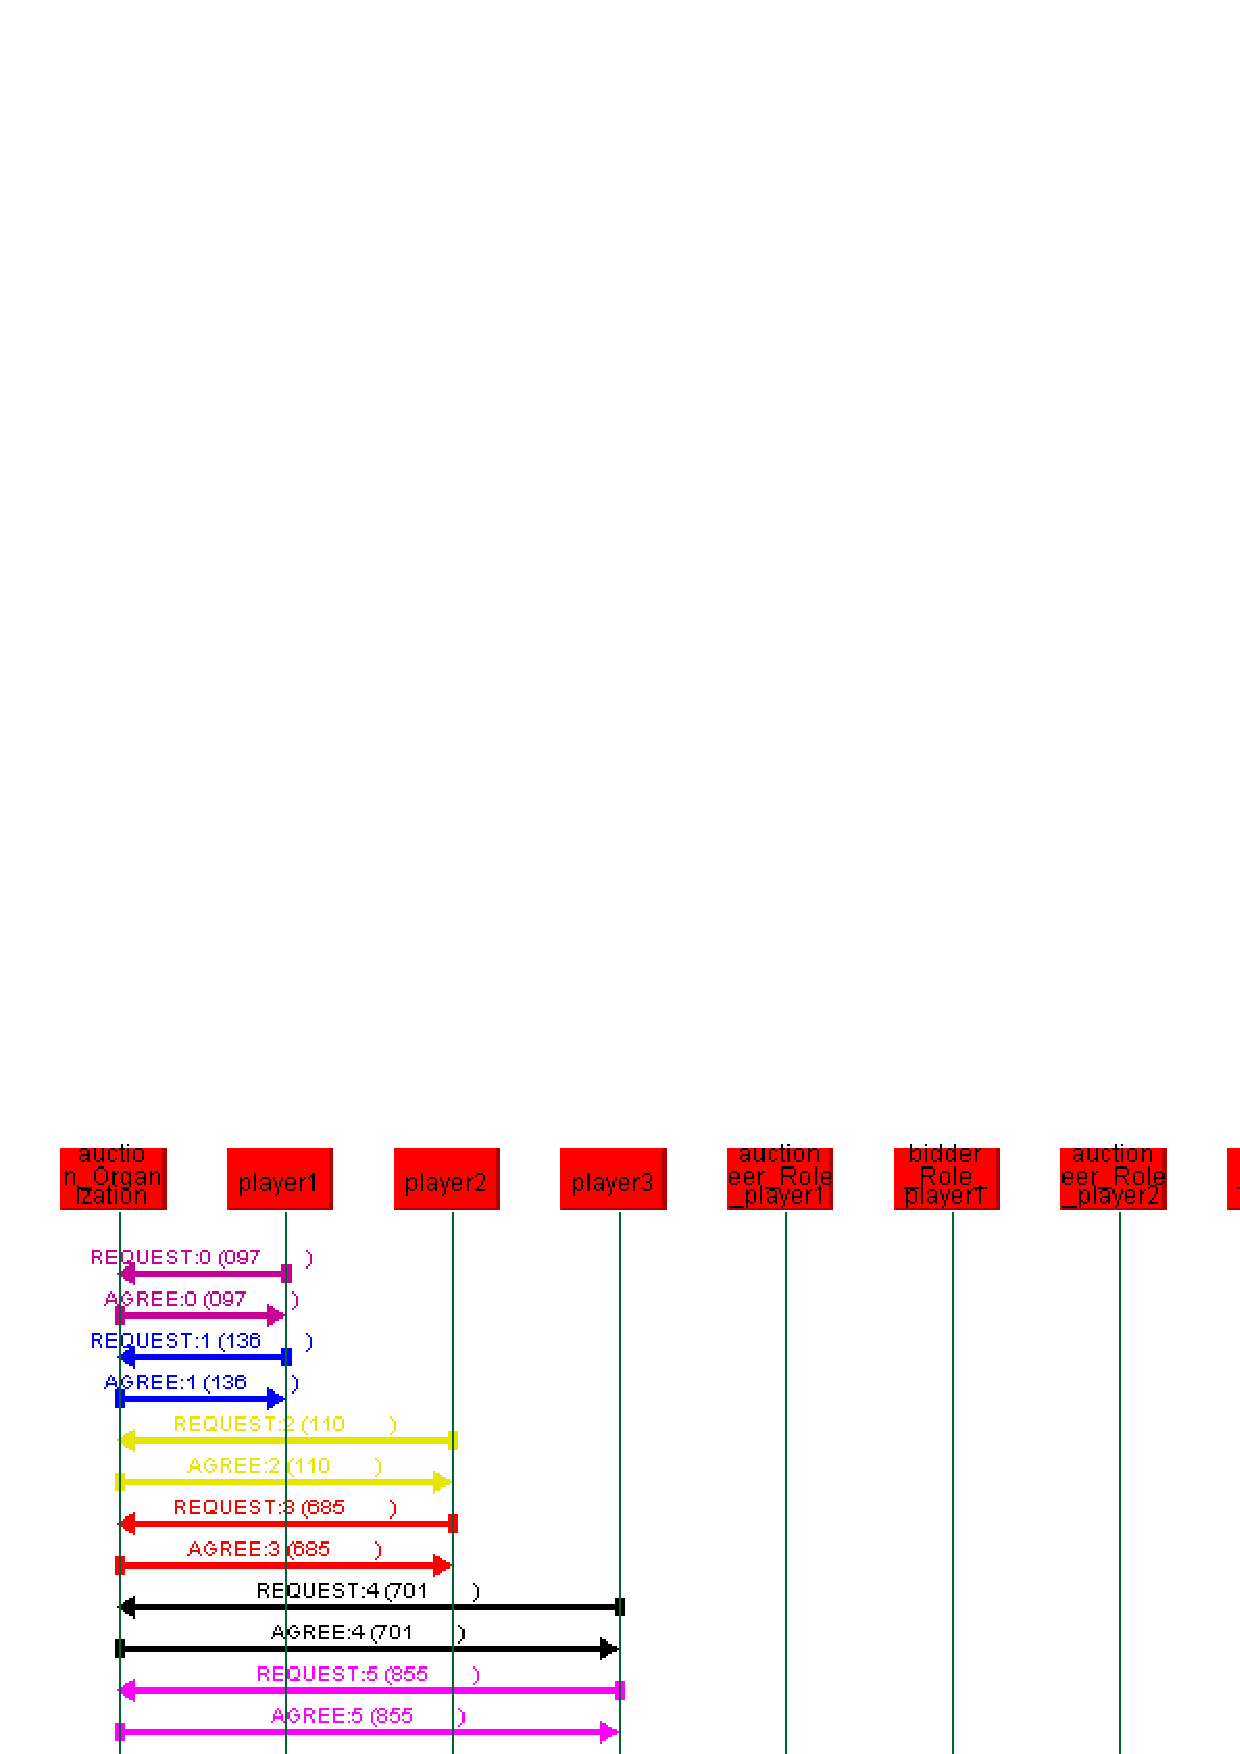
\includegraphics[width=\textwidth]{images/example3-stage5.png}
	\caption{Stage 5: Role deactment}
	\label{figure:example3-stage5}
\end{figure}

% Red
\textbf{Red} The red interaction scenario between the \textit{participant1} player and the \textit{auction} organization follows the \textit{Deact role} protocol.

% Magenta
\textbf{Magenta} The magenta interaction scenario between the \textit{participant2} player and the \textit{auction} organization follows the \textit{Deact role} protocol.
 
% Black
\textbf{Black} The black interaction scenario between the \textit{participant3} player and the \textit{auction} organization follows the \textit{Deact role} protocol.

% Deact role protocol - details
For details about the \textit{Deact role} interaction protocol see Stage 5 of the first example.